\documentclass[twoside,12pt,notitlepage]{Classes/CUEDthesisPSnPDF}

\defbibheading{bibliography}{\chapter{Bibliography}}
\bibliography{Dissertation/references}

\usepackage{appendix}
\usepackage{xcolor}
\usepackage{listings}
\usepackage{textcomp}

\usepackage{tikz}
\usetikzlibrary{shapes,arrows,positioning}

% Define block styles
\tikzstyle{decision} = [diamond, draw, %fill=blue!20,
    text width=4.5em, text badly centered, node distance=0.5cm, inner sep=0pt]
\tikzstyle{block} = [rectangle, draw, %fill=blue!20,
    text width=5em, text centered, rounded corners, minimum height=4em, node
    distance = 0.5cm]
\tikzstyle{block_spaced} = [rectangle, draw, %fill=blue!20,
    text width=5em, text centered, rounded corners, minimum height=4em, node
    distance = 1cm]
\tikzstyle{line} = [draw, -latex']
\tikzstyle{cloud} = [draw, ellipse, %fill=red!20,
    node distance=3cm, minimum height=2em]
\tikzstyle{decision answer}=[near start,color=black]


\raggedbottom                           % try to avoid widows and orphans
\sloppy
\clubpenalty1000%
\widowpenalty1000%

\addtolength{\oddsidemargin}{6mm}       % adjust margins
\addtolength{\evensidemargin}{-8mm}

\ifpdf
    \pdfinfo { /Title  (Docula - A Documentation Generation Engine)
               /Creator (TeX)
               /Producer (pdfTeX)
               /Author (Elliott Hillary <ejh67@cam.ac.uk>)
               /CreationDate (D:20121009000000)  %format D:YYYYMMDDhhmmss
               /ModDate (D:20121009000000)
               /Keywords (docula)}
    \pdfcatalog { /PageMode (/UseOutlines)
                  /OpenAction (fitbh)  }
\fi

% turn of those nasty overfull and underfull hboxes
\hbadness=10000
\hfuzz=50pt

% Comment out the next line to get single spacing
\onehalfspacing


\definecolor{solarized@base03}{HTML}{002B36}
\definecolor{solarized@base02}{HTML}{073642}
\definecolor{solarized@base01}{HTML}{586e75}
\definecolor{solarized@base00}{HTML}{657b83}
\definecolor{solarized@base0}{HTML}{839496}
\definecolor{solarized@base1}{HTML}{93a1a1}
\definecolor{solarized@base2}{HTML}{EEE8D5}
\definecolor{solarized@base3}{HTML}{FDF6E3}
\definecolor{solarized@yellow}{HTML}{B58900}
\definecolor{solarized@orange}{HTML}{CB4B16}
\definecolor{solarized@red}{HTML}{DC322F}
\definecolor{solarized@magenta}{HTML}{D33682}
\definecolor{solarized@violet}{HTML}{6C71C4}
\definecolor{solarized@blue}{HTML}{268BD2}
\definecolor{solarized@cyan}{HTML}{2AA198}
\definecolor{solarized@green}{HTML}{859900}

\lstdefinelanguage{treetop}[]{ruby}{
  morekeywords={rule},
  morecomment=[s]{<}{>}
}

\lstset{
    upquote=true,
    columns=fixed,
    tabsize=4,
    extendedchars=true,
    breaklines=true,
%    numbers=left,
    numbersep=5pt,
%    backgroundcolor=\color{solarized@base2},
    rulesepcolor=\color{solarized@base03},
    numberstyle=\tiny\color{solarized@base01},
    basicstyle=\footnotesize\ttfamily,
    keywordstyle=\color{solarized@green},
    stringstyle=\color{solarized@cyan}\ttfamily,
    identifierstyle=\color{solarized@blue},
    commentstyle=\color{solarized@base01},
    emphstyle=\color{solarized@red},
    showstringspaces=false
}

\lstnewenvironment{code}[1][]%
{
   \noindent
   \minipage{\linewidth}
   \vspace{0.5\baselineskip}
   \lstset{basicstyle=\ttfamily\footnotesize,#1}}
{\endminipage\vspace{0.5\baselineskip}}

\begin{document}

\pagestyle{empty}

\hfill{\LARGE \bf Elliott Hillary}

\vspace*{60mm}
\begin{center}
\Huge
{\bf Docula - A Documentation Generation Engine} \\
\vspace*{5mm}
Computer Science: Part II\\
\vspace*{5mm}
Girton College \\
\vspace*{5mm}
\today  % today's date
\end{center}

% set the number of sectioning levels that get number and appear in the contents
\setcounter{secnumdepth}{3}
\setcounter{tocdepth}{3}

\frontmatter % book mode only
\pagenumbering{roman}
\cleardoublepage
\chapter*{Proforma}

{\large
\begin{tabular}{ll}
Name:               & \bf Elliott Hillary                       \\
College:            & \bf Girton College                     \\
Project Title:      & \bf Docula - A Documentation Generation Engine \\
Examination:        & \bf Computer Science - Part II, July 2013        \\
Word Count:         & \bf 9001                             \\
Project Originator: & Elliott Hillary                    \\
Supervisor:         & Dr R.~Watts                   \\
\end{tabular}
}

\section*{Original Aims of the Project}



\section*{Work Completed}



\section*{Special Difficulties}


\cleardoublepage
\include{Dissertation/declaration}

\tableofcontents

\mainmatter % book mode only
\pagestyle{fancy}
\pagenumbering{arabic}
% The Introduction should explain the principal motivation for the project.
% Show how the work fits into the broad area of surrounding Computer Science and
% give a brief survey of previous related work. It should generally be
% unnecessary to quote at length from technical papers or textbooks. If a simple
% bibliographic reference is insufficient, consign any lengthy quotation to an
% appendix.

\chapter{Introduction}
Whilst working on several large projects, I have noticed the difference good
documentation can make to the further development or maintenance of a code base.
Documentation can save hours of tedious work finding the areas of the source
code that require work, without even considering the benefits it also brings by
better informing the developer about the inner workings of the code itself. Good
documentation informs the reader of what a particular section of code does and,
depending on the situation, what design decisions were made and how the code
itself works. When written properly, documentation should inform the reader in
enough detail that they can begin using the code without having to dig into its
internals.

The problem with writing good documentation is that it requires developer time
and skill to maintain, unfortunately most developers have neither. Documentation
generation helps to solve this problem, by minimising the amount of work a
developer has to do to produce documentation, meaning that they are more likely
to create useful documentation. First and foremost, documentation generation
allows for developers to write documentation in the source files themselves,
where it is later extracted by the generation software; this means that the
documentation is much more convenient to write, since it can be written
alongside the code. One additional benefit of this is that the generation
software can extract the information about the section being documented, such as
its type, and include this information in the documentation itself; this reduces
the amount of work the developer has to do, whilst also making it harder for the
documentation to become inconsistent with the code.

Software, such as doxygen\cite{website:doxygen} and
Javadoc\cite{website:javadoc}, already exists to perform these tasks and goes a
long way to making the lives of developers easier. These pieces of software, and
their alternatives, are widely used, but they offer an incomplete solution to
the problems they address; they focus on helping developers establish
\emph{what} a particular entity does, or is used for, but they do not try to
document the design decisions that led to this implementation nor the
considerations that drove them.

The intention of my project was to address these shortcomings.

% Principally, this chapter should describe the work which was undertaken before
% code was written, hardware built or theories worked on. It should show how the
% project proposal was further refined and clarified, so that the Implementation
% stage could go smoothly rather than by trial and error.

% Throughout this chapter and indeed the whole dissertation, it is essential to
% demonstrate that a proper professional approach was employed.

% The nature of this chapter will vary greatly from one dissertation to another
% but, underlining the professional approach, this chapter will very likely
% include a section headed "Requirements Analysis" and incorporate other
% references to the techniques of Software Engineering.

% The chapter will cite any new programming languages and systems which had to
% be learnt and will mention complicated theories or algorithms which required
% understanding.

\chapter{Preparation}
Before I can begin to write any code for this project, I first need to decide on
the components that will make up the core of it and ensure that any work that
needs to be done before code writing commences is completed. First step in this
is to define an overall structure to the project.

\begin{center}
  \vspace*{5mm}
  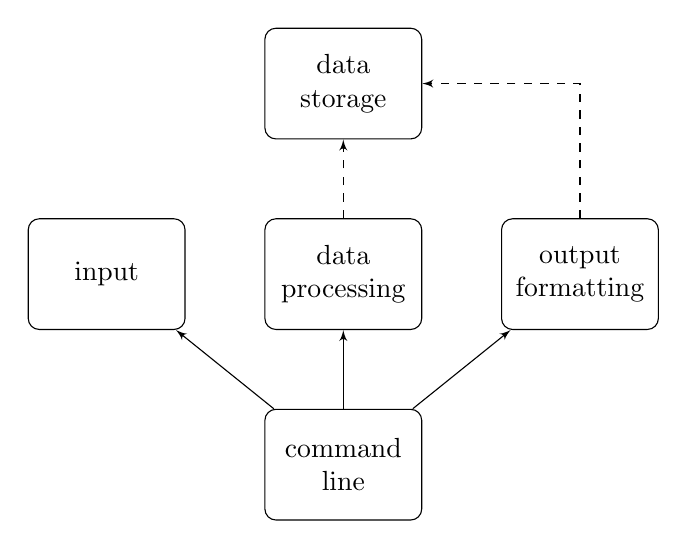
\begin{tikzpicture}[node distance = 2cm, auto]
    % Place nodes
    \node [block_spaced] (input) {input};
    \node [block_spaced, right=of input] (processing) {data processing};
    \node [block_spaced, above=of processing] (storage) {data storage};
    \node [block_spaced, right=of processing] (output) {output formatting};
    \node [block_spaced, below=of processing] (command) {command line};
    % Draw edges
    %\path [line] (input) -- (processing);
    %\path [line] (processing.100) -- (storage.260);
    %\path [line] (storage.280) -- (processing.80);
    %\path [line] (processing) -- (output);
    %\path [line] (storage.350) -| (output.100);
    %\path [line] (output.80) |- (storage.10);
    \path [line, dashed] (processing) -- (storage);
    \path [line, dashed] (output) |- (storage);
    \path [line] (command) -- (input);
    \path [line] (command) -- (processing);
    \path [line] (command) -- (output);
  \end{tikzpicture}
\end{center}

The command line component will act not only as an interface with the user, but
also interact with each of the input, processing \& output components, calling
them with the appropriate options and so on. This reduces coupling between the
other stages, since the command line component is the only one that needs
knowledge of all the stages, allowing for increased modularity of the code.

In addition to this structure, I also need to determine which language is the
appropriate choice for implementing this project, since each will have their own
strengths \& weaknesses, and how I will go about testing that everything is
working as it should along the way. While deciding on testing strategies before
programming is not required, it is important to test at some point in
development (whether it be throughout, at the end or both) and deciding on it
beforehand ensures that it will not be neglected.

I will be following the waterfall model of development for this project, as far
as is sensible, as maintenance is outside the scope of this project.

\section{Requirements Analysis}
This project consists of five parts:
\begin{itemize}
  \item One or more parsers, to transform the code base into an appropriate data
    structure.
  \item Code to process the above data structure and extract the required
    information from the code.
  \item Storage of the intermediate data.
  \item Code to transform the intermediate data into one or more human-readable
    formats.
  \item A command line interface, for use by the user.
\end{itemize}

For the purposes of this project, I will only be implementing a parser for one
programming language, since I believe that implementing more than one parser
would be a poor use of time \& resources and is beyond the scope of this
project. It will need to be a simple, standardised language to be completed in
the time available, there should also be sufficient code available written in
the language to provide thorough test cases. I have chosen to implement the
parser for C, as fulfils these requirements well.

Likewise, I will be implementing one concrete output format for the program; the
format should be one I am already familiar with and should easily support
linking between sections. I have decided that HTML is the best fit for the
output format, since it is easy to create \& does not require any extra tools to
generate or view the final result.

Even though I am only implementing one of each of the above stages, this does
not mean that I will be designing this software without other input \& output
formats in mind; the software should be developed with a view to be expanded in
the future, and therefore should be coded to be as modular as possible.

Strictly speaking, no storage of data is required, but adding this as a
component of the project does allow for us to improve the runtime of the
process. This can be done by determining whether a file has changed since it was
last parsed, if it has not there is no need to reinterpret the file, we can
simply use the data that is already stored about it. This is particularly
useful, as it will allow for quick incremental generation of the documentation,
so developers using the program will find it much more convenient to quickly use
to check that their documentation is in order.

\section{Comment Format}
In order to produce documentation from source code I need to define what
constitutes documentation, both so that I can parse \& process it and so that
appropriate documentation is actually written. This means defining a comment
format, I have previously used both Javadoc \& doxygen and have reviewed them
again prior to beginning this project. I have therefore kept their functionality
and limitations in mind while designing the comment format.

In my proposal, I specifically mentioned the compatibility with existing comment
formats was highly important to produce a useful result; as such, consideration
about the format I was going to be using had to be undertaken before any work
could begin. Both doxygen and Javadoc's comment formats are similar to one
another, and together they have quite a large market share, so it was sensible
to design a format that was compatible with these as much as possible. Ideally,
my format should be equal to or a superset of their formats, so that any
comments written with them in mind will work with the software I write.

With that in mind, I designed a format along the following lines (a full version
of which can be found in the appendix):

\begin{lstlisting}[language=c, escapechar=~]
  /**
   * Summary
   *
   * Full Description
   *
   * ~{\color{solarized@cyan} @param[in, out]}~ ptr Description of parameter ptr
   * ~{\color{solarized@cyan} @param[in]}~ size Description of parameter size
   * ~{\color{solarized@cyan} @return}~ Description of return value.
   */
  void *realloc(void *ptr, unsigned int size);
\end{lstlisting}

\begin{itemize}
  \item The first paragraph (i.e.~up to the first empty line) is considered to
    be a summary, and gives a brief outline of the intended use. This is
    standard practice with Javadoc, and can be enabled in doxygen.
  \item The following paragraphs make up the full description, expanding on the
    summary, describing in more detail what it does and how it should be used.
  \item @-annotations
    \begin{itemize}
      \item \lstinline|@param| annotations are used to describe the individual
        parameters and their purpose.
      \item The square-bracket suffixes to \lstinline|@param| annotations are
        for describing the flow of data, that is whether the variable is only
        used for input, output or both. These are described as \lstinline|[in]|,
        \lstinline|[out]| \& \lstinline|[in,out]| respectively. If a parameter
        is absent a flow annotation, it will be assumed that it is
        \lstinline|[in]|.
        doxygen already uses this way of describing flows; Javadoc does not have
        any such feature.
      \item \lstinline|@return| is used to describe what will be returned by the
        function; this may include under what conditions it will return an error
        and what those error values may be.
    \end{itemize}
    \item Summary \& Description sections can be applied to things other than
      functions, the @-annotations cannot, as they would be meaningless.
\end{itemize}

\section{Tools}
  \subsection{Programming Language}
    I opted to use Ruby to implement this project, whilst I do not have as much
    experience with Ruby as some other languages (like Java), I felt it was best
    suited to the project. Since one of Ruby's strengths is in its powerful
    text-manipulation capabilities it is well suited to this project, whereas
    processing Strings in Java can be quite heavyweight in terms of memory.

    Additionally, having looked into implementing parsers in various languages,
    I found that Treetop\cite{website:treetop} was well-suited to my needs.
    Treetop is a domain-specific language for Ruby, that facilitates the
    creation of parsing expression grammars; one of the particularly useful
    things about Treetop is that it allows you to define specific types for
    matched rules to instantiate, so that a lot of the effort of having to walk
    a parse tree can be alleviated. This will be discussed in further detail in
    the Implementation chapter.

    I was already partially familiar with Ruby, however I made use of
    \emph{Eloquent Ruby}\cite{book:eloquent_ruby} to further hone my knowledge
    of the language.
  \subsection{Version Control}
    Given that I have more previous experience with git than with any other
    version control system, I have decided to use it to manage my project. It
    provides additional advantages over some other version control systems,
    particularly in the fact that it is distributed; which means that the entire
    development history of the project will be available to me, no matter what
    machine I am working on.

    Using git will also allow me to make use of both GitHub and the PWF as a
    means of backup by pushing my changes to them regularly. As an additional
    form of backup my main development machine is backed up using OS X's Time
    Machine.

\section{Testing}
The testing of the project will be split in to two parts; part of it,
particularly in the development of the parser, will be performed during
development and the rest will be performed after the completion of the main
body of the code has been written.

  \subsection{Regression Testing}
    In order to implement the parser successfully, I will be making use of
    regression testing; this will be used to ensure that the parser behaves
    in an expected manner for specific inputs, and make sure that when new
    functionality is added it does not fail any of the previous tests.

    To do this I will be writing short snippets of code that implement a
    specific part of the language's feature set, and then making sure that these
    tests pass before continuing, such as:

    \begin{lstlisting}[language=c, gobble=4]
      int c;
    \end{lstlisting}

    This makes sure that I identify bugs early, and prevents me from introducing
    any new ones later in development, allowing me to fix them before they cause
    any serious problems.

  \subsection{End Testing}
    Evaluating documentation is inherently a subjective process, and so it would
    not be feasible to evaluate by any formal means; as such, I will be creating
    a questionnaire which will be given to several members of staff at
    Dr.~Watts' company, along with the software itself, for them to evaluate
    compared to their usual documentation solutions. This questionnaire, and any
    familiarisation with the software required, should take no longer than half
    an hour; to take any longer is unnecessary, as it is initial opinions which
    will ultimately decide someone's choice of whether or not to use the
    software, and so I would like to attempt to capture that within the survey.

    In order for the surveys to be completed the documentation software will
    have to be used on a sample of code from the workplace ensuring that it
    functions across a wide spectrum of styles and is therefore suitable for use
    in the working environment.

% \section{Action Plan}
% I then created an action plan with these main aims in mind in order to ensure
% the project's success; I will be be adopting the waterfall model to develop this
% project, and so the plan follows that general structure.
% \begin{enumerate}
%   \item Research - look at existing documentation software, and identify their
%     flaws \& attributes.
%   \item Identify the features required in this parser, taking into account the
%     strengths \& weaknesses identified in the previous phase to determine the
%     functionality to be included or improved upon.
%   \item Develop an outline for the project so that an awareness of structure and
%     flow can form. Plan what order the code shall be written in and what order -
%     what tests need to be performed along the way to ensure functionality.
%   \item Choose the programming language best suited to the project - learn
%     and/or practise the language to ensure fluency and suitability for the
%     project.
%   \item List and develop tests that will take place during the coding and at the
%     end to ensure the project functions correctly.
%   \item Begin writing and testing code - revisit plan if necessary to make
%     alterations.
%   \item Complete end testing and make any necessary alterations
% \end{enumerate}

% This chapter should describe what was actually produced: the programs which
% were written, the hardware which was built or the theory which was developed.
% Any design strategies that looked ahead to the testing stage might profitably
% be referred to (the professional approach again).

% Descriptions of programs may include fragments of high-level code but large
% chunks of code are usually best left to appendices or omitted altogether.
% Analogous advice applies to circuit diagrams.

% Draw attention to the parts of the work which are not your own. Making
% effective use of powerful tools and pre-existing code is often laudable, and
% will count to your credit if properly reported.

% It should not be necessary to give a day-by-day account of the progress of the
% work but major milestones may sometimes be highlighted with advantage.

\chapter{Implementation}

\section{The Parser}
To implement my parser, I made use of an existing domain-specific language
available as a Ruby library called Treetop\cite{website:treetop}; Treetop allows
for easy implementation of Parsing Expression Grammars, which, simply put, are
grammars that built up out of a combination of rules and regular expressions.

Parsing Expression Grammars were particularly appealing to me for two reasons:
firstly, they are essentially a more powerful version of regular expressions,
with which I am already familiar and secondly, they can be made to run in
constant time if implemented as a packrat parser, which Treetop does. This
constant time guarantee is provided by the process of memoization, which trades
off time for space by caching previous inputs and the resulting parse trees to
remove the need for repeated computations.

Treetop grammars are written as their own .treetop files, which are then used
to generate the parsers by the \lstinline|tt| program. The end result is a Ruby
source file which can be included and used to parse the language defined by the
grammar. Treetop also allows you to define a class that nodes within the parsed
data should be instantiated as, this means that nodes can be given methods with
which they can parse themselves or their children; which is much preferable to
the traditional methods of writing code to walk the tree structures.

\begin{code}[language=treetop]
  rule comment
    '//' ( !EOL .)* EOL <CommentNode>
    / '# ' ( !EOL .)* EOL <CommentNode>
    / (multiline_comment) <CommentNode>
  end
  rule multiline_comment
    '/*'
    (
      !'*/'
      (. / EOL)
    )*
    '*/'
  end
  rule EOL
    [\n]
  end
\end{code}

Above is a snippet from my Treetop grammar for C, defining the grammar for
comments. The rule \lstinline|comment| contains an ordered choice of expressions
that define each type of comment available in C, and informs Treetop that they
should be instantiated using the class \lstinline|CommentNode|;
\lstinline|CommentNode| defines a method with which the text of the comment
can be extracted.


  \subsection{Regression Testing}
    To ensure that I was properly implementing my grammar for C, I wrote some
    tests for my parser that would check that parsing a particular piece of code
    would yield a valid result. This was the quickest \& easiest way of building
    up a working grammar for the language and allowed me to be confident that
    what I had written would function correctly as I moved forward.

    This was implemented using \lstinline|TestCase|, a class that is part of the
    Ruby standard library, and simply involves defining methods that execute the
    code required for each test and uses various types of assertions to ensure
    that the results are as expected.

    The process went as follows:

    \begin{center}
    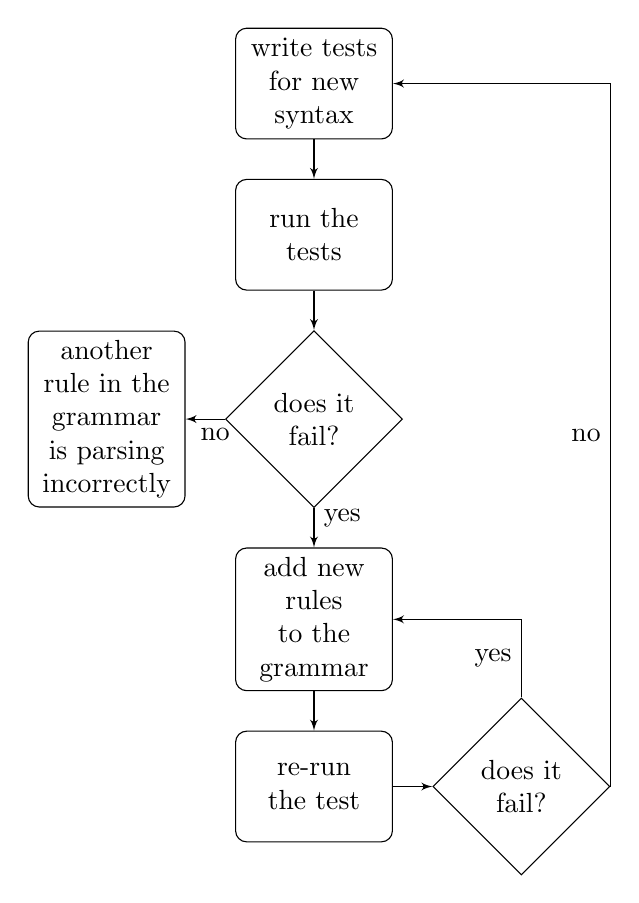
\begin{tikzpicture}[node distance = 2cm, auto]
        % Place nodes
        \node [block] (init) {write tests for new syntax};
        \node [block, below=of init] (run) {run the tests};
        \node [decision, below=of run] (fail) {does it fail?};
        \node [block, left=of fail] (debug) {another rule in the grammar is
          parsing incorrectly};
        \node [block, below=of fail, node distance=3cm] (develop) {add new rules
          to the grammar};
        \node [block, below=of develop, node distance=3cm] (rerun) {re-run the
          test};
        \node [decision, right=of rerun] (refail) {does it fail?};
        % Draw edges
        \path [line] (init) -- (run);
        \path [line] (run) -- (fail);
        \path [line] (fail) -- node[decision answer] {no} (debug);
        \path [line] (fail) -- node[decision answer] {yes} (develop);
        \path [line] (develop) -- (rerun);
        \path [line] (rerun) -- (refail);
        \path [line] (refail.east) |- node[decision answer] {no} (init);
        \path [line] (refail) |- node[decision answer] {yes} (develop);
    \end{tikzpicture}
    \end{center}

  \subsection{Parsing Problems}
    As I wrote my initial grammar for the C parser, it became apparent that I
    was having some problems; I got to the point where implementing new rules
    within the grammar would cause other tests to fail, the problem was that
    describing C correctly required such a huge grammar that the rules were
    interacting in ways I had not accounted for. This meant that progress on the
    grammar slowed to a crawl, and it became apparent that the grammar would
    need to be largely rethought to fully parse C.

    I realised, however, that in order to parse C for the purposes of generating
    documentation, I did not need my parser to completely understand the
    language, instead it needed to only understand enough to parse to top level.
    I therefore wrote a new, simpler parser that understood how to navigate
    through the C files, rather than parsing all of it; this brought an added
    advantage of improving the runtime of the parser.

    Instead of parsing function bodies, the simplified parser contains rules to
    match pairs of braces within functions, ignoring those in strings and
    comments, to understand where functions begin \& end. With global variable
    assignments, the parser has rules to match from an equals sign to the
    semicolon at the end of the line. These simplifications allowed for me to
    dispense with the expensive and complicated parsing of control structures
    and arithmetic, and reduced the grammar from ${\sim}$500 lines in the
    original (unfinished) grammar to ${\sim}$300 lines for the completed
    simplified one.

    Ideally, some or all of the more complex behaviour would be restored to the
    grammar, as it would allow for better analysis of the parsed language, such
    as including in the documentation what was referenced by a particular
    function. Given the time constraints involved in the project, this could not
    be performed.

\section{Handling the Data}
After the source files have been parsed into a parse tree, the useful data can
be extracted; using the methods that were added into the parse tree by Treetop,
the code runs through the functions, variables \& other pieces of data and pulls
out the needed information to be stored in the database.

To store the data I opted to use SQLite, as it requires no configuration to use
and stores all data in a file, rather than on a SQL server; this means that no
setup of databases is required on the part of the user. I used the
sqlite3\cite{website:sqlite} Ruby library to interact with my database, which
allows you to interact with data from the database using the normal Ruby types.

  \subsection{Processing}
    The classes I defined for use in the parse tree provide easy access to the
    data within the nodes, and their subtrees, whilst masking the specifics of
    the tree itself; this means that future additions to the parser and the way
    in which it works will not affect the processing of the data. In addition,
    this allows for the reuse of the processing code on the parse trees of
    different languages, provided that the nodes in that tree expose the same
    methods.

    Since some functions in the source being parsed may only be partially
    documented, I needed to account for this in my code to ensure that the
    resulting data was consistent; in particular, if a function is documented
    the hash containing information about the prototype will contain extra
    information. Uniting the arguments with their documentation proved
    interesting, and I had to write the code for managing it several times
    before I created a solution that provided an appropriate output regardless
    of input.

    \begin{code}[language=ruby, gobble=6]
      if function.documented?
        prototype[:arguments] = prototype[:arguments].zip(prototype[:params]).map do |a,d|
          d ? a.merge(d) : a
        end
        prototype.delete(:params)
      end
    \end{code}

    This small section of code was the eventual solution, and in just a few
    lines accomplishes quite a bit. The array containing the arguments
    parsed, from the function prototype itself, is merged with the array
    containing the documentation for each argument, producing a new array. This
    array is contains several arrays, each holding the documentation and
    prototype for one argument; finally, the map function returns the array I
    need by merging the two hashes together, if the argument is documented, or
    returning the just the argument's hash if no documentation exists. The
    example data below demonstrates the process.

    \begin{code}[language=ruby, gobble=6]
      A = [{a => 1}, {b => 2}, {c => 3}]
      B = [{d => 4}, {}, {f => 6}]

      # After zipping A & B...

      C = [[{a => 1}, {d => 4}], [{b => 2}], [{c => 3}, {f => 6}]]

      # After mapping C...

      D = [{a => 1, d => 4}, {b => 2}, {c => 3, f => 6}]
    \end{code}

      \subsubsection{Post-processing}
        Once the data for all files in the directory has been added to the
        database, some extra processing takes place to resolve which files
        include one another. By looping through all the includes encountered
        and determining whether it refers another file that has been processed,
        links are built between files, which are later used by the output stage
        to allow a user to jump from one file to one of its includes easily.

        To determine if one file refers to another, I decided to check whether a
        following the path described in the include exists, relative to that
        file. This is by no means a fool-proof solution, as it does not take
        into account the include paths passed to a compiler, but the only other
        sensible solution to this problem would be to also parse the Makefile
        (or similar file in another build system) to extract the include paths
        used. Given the number of different build systems used and the time
        taken to implement another grammar for parsing any of them, I concluded
        that this was not a valid solution in the time available.

  \subsection{Storage}

    \subsubsection{Foreign Keys}

\section{Generating the Output}

\section{The Command-Line Interface}

  \subsection{Option Parsing}

% This is where Assessors will be looking for signs of success and for evidence
% of thorough and systematic testing. Sample output, tables of timings and
% photographs of workstation screens, oscilloscope traces or circuit boards may
% be included.

% As with code, voluminous examples of sample output are usually best left to
% appendices or omitted altogether.

% There are some obvious questions which this chapter will address. How many of
% the original goals were achieved? Were they proved to have been achieved? Did
% the program/hardware/theory really work?

% Assessors are well aware that large programs will very likely include some
% residual bugs. It should always be possible to demonstrate that a program
% works in simple cases and it is instructive to demonstrate how close it is to
% working in a really ambitious case.

\chapter{Evaluation}

\section{Speed Testing}
An important aspect of this project is speed, this is because users will not
want to wait excessive lengths of time for the tool to complete, particularly if
it is expected to be used incrementally, as this is. In order to test this, I
ran the software over several open-source projects and measured their runtime;
as a comparision, I also used doxygen on the same projects. As my project stores
information from files so that future runs are quicker, I ran the tool a second
time over the source trees to examine how much effect this has; doxygen does not
do any such storing, and so only one execution was required per project.

In the interests of ensuring that the measurements were correct, this process
was performed several times for each project, and the results were averaged. In
each case, results were pretty consistent.

Since the software failed on some source files due to problems with my parser,
not all files were successfully parsed; to account for this, I decided to
estimate the total time the software would have taken. When the parser fails,
the line on which it failed can be retrieved, I used this to determine the
fraction of the file that was successfully parsed and estimated the time that
would be taken. This allows for a fairer comparison with doxygen.

\noindent\makebox[\textwidth]{%
  \includegraphics[width=160mm]{Graphs/timings.pdf}
}

Above is a graph comparing the execution times of my project \& doxygen, the
bars for my software are broken down into three parts: the actual runtime,
projected runtime, and the time for a subsequent run.

These results demonstrate that doxygen is generally faster than my software on
the first run, even without accounting for the failed files; however, in all but
one test, my software out-performs doxygen on subsequent runs. These results are
fairly in-line with my expectations: doxygen is written in C++ and therefore has
less of an overhead compared to my solution, not to mention that its developers
have had much longer to tune the performance of their software. I had also
expected that my use of a database would allow for a dramatic increase in speed,
and I am pleased to see that this was the case.

  \subsection{Profiling}
  In addition to running the above tests, I also opted to profile the code to
  try and work out what sections were causing the high execution times. I had
  expected to find that the I/O to the database on disk was the cause of it, but
  the results of profiling demonstrated that the parser was in fact the slowest
  component; in particular, the sheer number of classes that Treetop
  instantiated caused calls to \lstinline|Class#new| and
  \lstinline|Kernel#extend| to take a significant proportion ($\sim$8\%) of the
  total execution time!

  Upon further investigation I discovered why Treetop was instantiating so
  many classes, it would appear that any match to part of a defined rule
  creates a \lstinline|SyntaxNode|. The rules for defining comments illustrate
  this problem well: part of its definition contains ``\lstinline|( !EOL .)*|''
  which matches any character other than a newline, causing a
  \lstinline|SyntaxNode| to be created for \emph{every character in the
  comment}. Fortunately, this means that the parser's performance could be
  improved with better regular expressions.



% This chapter is likely to be very short and it may well refer back to the
% Introduction. It might properly explain how you would have planned the project
% if starting again with the benefit of hindsight.

\chapter{Conclusion}
I have successfully produced software capable of transforming source code, using
appropriately-styled comments, into human-readable documentation. The software
does not completely parse the C language correctly, mainly due to difficulties
in parsing preprocessor macros; given more time, this should be fairly easy to
fix. As the results in the previous chapter show, the software parses source
trees faster on subsequent runs than doxygen, due to the use of persistent
storage.

Whilst the software I have produced does indeed produce documentation, it does
not address the shortcomings that I identified in existing documentation
generation software, namely that they do not allow the developer to fully
describe ``the design decisions that led to this implementation nor the
considerations that drove them''. Due in part to time constraints, difficulties
and hold-ups in the implementation process, the software I have produced only
goes as far as existing software does in displaying documentation, however I
believe that I have designed my system in a modular enough way that these things
could be added in the future without any significant re-designs taking place.

I originally opted to use Treetop for creating the parser because it allowed me
to implement it in a way that was logical and familiar to me, with hindsight, it
would perhaps have been better (at least, in the time that was available to me)
to make use of an infrastructure such as LLVM\cite{website:llvm} to facilitate
the parsing. This would have also given me the added advantage of being able to
perform some static analysis on the code, potentially allowing for the generated
documentation to display information about the usage of functions. The downside
to this is that LLVM would only be usable with languages that have a front-end
implemented for it, whereas Treetop could be used to parse any language. With
hindsight, I would have at least considered using LLVM instead of, or in
combination with, Treetop to do my parsing.

Overall I believe that my project was a modest success, despite not doing
everything I set out to do, it does go a long way to being a competent
documentation generator.


\printbibliography

\begin{appendices}
\chapter{Comment Format}

\begin{lstlisting}[language=c,gobble=4]
    /**
     * In order to ensure compatibility with Doxygen, I needed to
     * create a comment format that was as similar to theirs as
     * possible.
     * Any block comment with a double star opening will be
     * considered for a documentation string.
     */

     /// Triple slashes opening a single line are also considered.

     /**
      * Documentation immediately preceding a function definition
      * will become associated with that function.
      *
      * Typically, the first paragraph is a summary, with the
      * subsequent paragraphs providing greater detail; this can
      * be disabled in the options.
      *
      * @param[in] Description of first argument
      * @param[inout] Description of second argument
      * @return Description of return value
      * @error Describes what make be returned in the case of an
      *        error.
      *
      * The @param annotations are for describing the arguments
      * passed into the function - what they represent and/or the
      * range or valid values - they also specify whether the
      * argument is used solely for input, output, or both
      * ([in], [out] and [inout], respectively).
      */
    int example(int arg1, char* arg2);

    /// Documentation may also precede variables...
    int important_var;

    /// ... Or even #defines.
    #define ULTIMATE_ANSWER 42

    /**
     * @file
     *
     * Documentation marked with the @file annotation denote that
     * they are referring to the file as a whole.
     *
     * These comments may also include other relevant information,
     * such as:
     * @copyright My Company Inc.
     * @author Elliott Hillary
     * @created 2012-10-18
     */
\end{lstlisting}

\chapter{Project Proposal}
\section{Introduction, The Problem To Be Addressed}

In the development and maintenance of software, especially those
containing large amounts of code, documentation frequently becomes a
problem. Often documentation is written separately from the code
itself, and as such the two diverge over time, leaving maintainers
worse of than they'd never checked both in the first place. It is the
aim of this project to tackle this problem and to facilitate not only
the writing of correct and thorough documentation, but also the easy
maintenance of both code and documentation; this is to be achieved by
defining a syntax to interleave code with documentation, so that both
are kept together and so are more easily kept in synchronisation with
one another.

It is important to distinguish between the two types of documentation
that occur in software development\footnote{The naming of these is
purely of my own invention, and as far as I'm aware is not part of any
established convention; I will, however, be using these names
throughout.} Together, these two types of documentation should
describe a piece of software thoroughly:

\begin{description}
\item[Interface documentation] essentially defines a contract with the
  outside world as to what this function or class does, what it
  expects as input to give a valid output, what may (or may not)
  happen when given invalid inputs, and so on.

  It is important that \emph{interface documentation} be well-defined,
  as it is what informs another developer now or in the future as to
  what the function is \emph{supposed} to do.

\item[Implementation documentation] is essentially the comments that
  developers put (or rather, should put) into their code that explains
  \emph{how} and \emph{why} they are doing things the way they're
  doing them. These comments should be written with the expectation
  that someone else in the future may actually be using them to track
  down the relevant piece of code they looking to fix or update, as
  such they should be written as proper sentences and written in such
  a way that the comments can be combined into a full document that
  talks its way through the function.

  The \emph{implementation documentation} does not need to be as
  strictly defined as the \emph{interface documentation}, as it is
  more a process of describing the choices made in writing the
  function, rather than its intended use.
\end{description}

\section{Starting Point}

Several other documentation engines exist, such as Doxygen \& Javadoc,
however none of them seem to account for the two distinct types of
documentation that exist within a code base. I have used both Doxygen
\& Javadoc to document projects in the past, and so I am familiar with
the style in which the comments used for the documentation are
written.

Since that there is already wide use of these, particularly Doxygen,
I will be designing my syntax to be as compatible with theirs as
possible. This will allow users to easily switch between the two and
allow for increased uptake of the engine.

\section{Resources Required}

I shall be primarily be using my own computer for the development of
this project, which is currently a laptop running Mac OS X; I will
also be using the PWF machines, to ensure that the software produced
runs across a variety of UNIX-like operating systems. The project
shall be backed up to a git repository on BitBucket, and also to the
PWF.

I require no other special resources.

\section{Work to be done}

{\em Describe the technical work.}

The project breaks down into the following sub-projects:

\begin{enumerate}

\item The construction of a skeleton dissertation with the required 
structure. This involves writing the Makefile and makeing dummy files
for the title page, the proforma, chapters 1 to 5, the appendices and
the proposal.

\item Filling in the details required in the cover page and proforma.

\item Writing the contents of chapters 1 to 5, including examples
of common \LaTeX\ constructs.

\item Adding a example of how to use floating figures and encapsulated
postscript diagrams.

\end{enumerate}

\section{Success Criterion for the Main Result}


The project will be a success if I have a completed dissertation with the correct chapter
titles and I have achieved my other success criterion, which is to blah ...



\section{Possible Extensions}

{\em Potential further envisaged evaluation metrics or extensions.}

If I achieve my main result early I shall try the following alternative experiment or method of evaluation ...


\section{Timetable: Workplan and Milestones to be achieved.}


{\em Perhaps list ten or so  two-week work-packages.}

Planned starting date is 16/10/2011.

\begin{enumerate}

\item {\bf Michaelmas weeks 2-4} Learn to use X. Read book Y. Read papers Z.

\item {\bf Michaelmas weeks 5-6} Do preliminary test of Q.

\item {\bf Michaelmas weeks 7-8} Start implementation of main task A.

\item {\bf Michaelmas vacation} Finish A and start main task B.

\item {\bf Lent weeks 0-2} Write progress report. Generate corpus of test examples. Finish task B.  

\item {\bf Lent weeks 3-5} Run main experiments and achieve working project.

\item {\bf Lent weeks 6-8} Second main deliverable here.

\item {\bf Easter vacation:} Extensions and writing dissertation main chapters.

\item {\bf Easter term 0-2:}  Further evaluation and complete dissertation.

\item {\bf Easter term 3:} Proof reading and then an early submission so as to concentrate on examination revision.

\end{enumerate}


 


\end{appendices}

\end{document}
